\documentclass[12pt]{book}

\usepackage{xeCJK}
\usepackage{listings}
\usepackage{multirow}
\usepackage{longtable}
\usepackage{fontspec}
\usepackage{ctex}
\usepackage[top=3cm,bottom=3cm,left=3cm,right=3cm, headsep=10pt,a4paper]{geometry} % Page margins
\usepackage{graphicx} % Required for including pictures
\graphicspath{{Pictures/}{Image/common/}} % Specifies the directory where pictures are stored
\usepackage{lipsum} % Inserts dummy text
\usepackage[ddmmyyyy]{datetime}
\usepackage{tikz} % Required for drawing custom shapes
\usepackage[english]{babel} % English language/hyphenation
\usepackage{enumitem} % Customize lists
\setlist{nolistsep} % Reduce spacing between bullet points and numbered lists
\usepackage{booktabs} % Required for nicer horizontal rules in tables
\usepackage{xcolor} % Required for specifying colors by name
\definecolor{ocre}{RGB}{243,102,25} % Define the orange color used for highlighting throughout the book
\usepackage{avant} % Use the Avantgarde font for headings
%\usepackage{times} % Use the Times font for headings
\usepackage{mathptmx} % Use the Adobe Times Roman as the default text font together with math symbols from the Sym­bol, Chancery and Com­puter Modern fonts
\usepackage{microtype} % Slightly tweak font spacing for aesthetics
\usepackage[T1]{fontenc}
\usepackage[utf8]{inputenc}
{\renewcommand{\bibname}{References}}
\usepackage[backend=bibtex,style=numeric]{biblatex}

\defbibheading{bibempty}{}

\usepackage{calc} % 简单的计算功能
\usepackage{makeidx} % 创建索引
\makeindex % Tells LaTeX to create the files required for indexing
\usepackage{titletoc} % 目录操作
\usepackage[bookmarksopen,bookmarksdepth=3]{hyperref}


%When compile under liunx% 

%\setCJKmainfont{WenQuanYi Micro Hei} % 设置缺省中文字体

\contentsmargin{0cm} % Removes the default margin

\lstdefinelanguage{JavaScript}{
	keywords={typeof, new, true, false, catch, function, return, null, catch, switch, var, if, in, while, do, else, case, break},
	keywordstyle=\color{blue}\bfseries,
	ndkeywords={class, export, boolean, throw, implements, import, this},
	ndkeywordstyle=\color{darkgray}\bfseries,
	identifierstyle=\color{black},
	sensitive=false,
	comment=[l]{//},
	morecomment=[s]{/*}{*/},
	commentstyle=\color{purple}\ttfamily,
	stringstyle=\color{red}\ttfamily,
	morestring=[b]',
	morestring=[b]"
}

%Figure显示为中文的“图”
\renewcommand\figurename{图}

\setcounter{tocdepth}{2}

%Set Code Format%
\lstloadlanguages{C, csh, make,python,Java,JavaScript}
\lstset{	  
	alsolanguage= XML,  
	tabsize=4, %  
	frame=shadowbox, %把代码用带有阴影的框圈起来  
	commentstyle=\color{red!50!green!50!blue!50},%浅灰色的注释
	frameround=tttt,  
	rulesepcolor=\color{red!20!green!20!blue!20},%代码块边框为淡青色  
	keywordstyle=\color{blue!90}\bfseries, %代码关键字的颜色为蓝色,粗体  
	showstringspaces=false,%不显示代码字符串中间的空格标记  
	stringstyle=\ttfamily, % 代码字符串的特殊格式  
	keepspaces=true, %  
	breakindent=22pt, % 
	breaklines=true,%设置代码自动换行 
	numbers=left,%左侧显示行号 往左靠,还可以为right,或none,即不加行号  
	stepnumber=1,%若设置为2,则显示行号为1,3,5,即stepnumber为公差,默认stepnumber=1  
	%numberstyle=\tiny, %行号字体用小号  
	numberstyle={\color[RGB]{0,192,192}\tiny},%设置行号的大小,大小有tiny,scriptsize,footnotesize,small,normalsize,large等  
	numbersep=8pt,  %设置行号与代码的距离,默认是5pt  
	basicstyle=\ttfamily, % 这句设置代码的大小  
	showspaces=false, % 
	escapechar=`,
	flexiblecolumns=true, %  
	breaklines=true, %对过长的代码自动换行  
	breakautoindent=true,%  
	breakindent=4em, %  	   
	aboveskip=1em, %代码块边框  
	tabsize=4,  
	showstringspaces=false, %不显示字符串中的空格  
	backgroundcolor=\color[RGB]{245,245,244},   %代码背景色  
	%backgroundcolor=\color[rgb]{0.91,0.91,0.91}    %添加背景色  
	escapeinside={``}{\_},  %在``里显示中文  
	%% added by http://bbs.ctex.org/viewthread.php?tid=53451  
	fontadjust,  
	captionpos=t,  
	framextopmargin=2pt,
	framexbottommargin=2pt,
	abovecaptionskip=-3pt,
	belowcaptionskip=3pt,  
	xleftmargin=4em,
	xrightmargin=4em, % 设定listing左右的空白  
	texcl=true
}

% Part text styling
\titlecontents{part}[0cm]{\addvspace{20pt}\centering\large\sffamily}{}{}{}

% Chapter text styling
\titlecontents{chapter}[1.25cm] % Indentation
{\addvspace{12pt}\large\sffamily\bfseries} % Spacing and font options for chapters
{\color{ocre!60}\contentslabel[\Large\thecontentslabel]{1.25cm}\color{ocre}} % Chapter number
{\color{ocre}}  
{\color{ocre!60}\normalsize\;\titlerule*[.5pc]{.}\;\thecontentspage} % Page number

% Section text styling
\titlecontents{section}[1.25cm] % Indentation
{\addvspace{3pt}\sffamily\bfseries} % Spacing and font options for sections
{\contentslabel[\thecontentslabel]{1.25cm}} % Section number
{}
{\hfill\color{black}\thecontentspage} % Page number
[]

% Subsection text styling
\titlecontents{subsection}[1.25cm] % Indentation
{\addvspace{1pt}\sffamily\small} % Spacing and font options for subsections
{\contentslabel[\thecontentslabel]{1.25cm}} % Subsection number
{}
{\ \titlerule*[.5pc]{.}\;\thecontentspage} % Page number
[]

% List of figures
\titlecontents{figure}[0em]
{\addvspace{-5pt}\sffamily}
{\thecontentslabel\hspace*{1em}}
{}
{\ \titlerule*[.5pc]{.}\;\thecontentspage}
[]

% List of tables
\titlecontents{table}[0em]
{\addvspace{-5pt}\sffamily}
{\thecontentslabel\hspace*{1em}}
{}
{\ \titlerule*[.5pc]{.}\;\thecontentspage}
[]

%----------------------------------------------------------------------------------------
%	MINI TABLE OF CONTENTS IN PART HEADS
%----------------------------------------------------------------------------------------

% Chapter text styling
\titlecontents{lchapter}[0em] % Indenting
{\addvspace{15pt}\large\sffamily\bfseries} % Spacing and font options for chapters
{\color{ocre}\contentslabel[\Large\thecontentslabel]{1.25cm}\color{ocre}} % Chapter number
{}  
{\color{ocre}\normalsize\sffamily\bfseries\;\titlerule*[.5pc]{.}\;\thecontentspage} % Page number

% Section text styling
\titlecontents{lsection}[0em] % Indenting
{\sffamily\small} % Spacing and font options for sections
{\contentslabel[\thecontentslabel]{1.25cm}} % Section number
{}
{}

% Subsection text styling
\titlecontents{lsubsection}[.5em] % Indentation
{\normalfont\footnotesize\sffamily} % Font settings
{}
{}
{}

%----------------------------------------------------------------------------------------
%	PAGE HEADERS
%----------------------------------------------------------------------------------------

\usepackage{fancyhdr} % Required for header and footer configuration

\pagestyle{fancy}
\renewcommand{\chaptermark}[1]{\markboth{\sffamily\normalsize\bfseries\chaptername\ \thechapter.\ #1}{}} % Chapter text font settings
\renewcommand{\sectionmark}[1]{\markright{\sffamily\normalsize\thesection\hspace{5pt}#1}{}} % Section text font settings
\fancyhf{} \fancyhead[LE,RO]{\sffamily\normalsize\thepage} % Font setting for the page number in the header
\fancyhead[LO]{\rightmark} % Print the nearest section name on the left side of odd pages
\fancyhead[RE]{\leftmark} % Print the current chapter name on the right side of even pages
\renewcommand{\headrulewidth}{0.5pt} % Width of the rule under the header
\addtolength{\headheight}{2.5pt} % Increase the spacing around the header slightly
\renewcommand{\footrulewidth}{0pt} % Removes the rule in the footer
\fancypagestyle{plain}{\fancyhead{}\renewcommand{\headrulewidth}{0pt}} % Style for when a plain pagestyle is specified

% Removes the header from odd empty pages at the end of chapters
\makeatletter
\renewcommand{\cleardoublepage}{
	\clearpage\ifodd\c@page\else
	\hbox{}
	\vspace*{\fill}
	\thispagestyle{empty}
	\newpage
	\fi}

%----------------------------------------------------------------------------------------
%	THEOREM STYLES
%----------------------------------------------------------------------------------------

\usepackage{amsmath,amsfonts,amssymb,amsthm} % For math equations, theorems, symbols, etc

\newcommand{\intoo}[2]{\mathopen{]}#1\,;#2\mathclose{[}}
\newcommand{\ud}{\mathop{\mathrm{{}d}}\mathopen{}}
\newcommand{\intff}[2]{\mathopen{[}#1\,;#2\mathclose{]}}
\newtheorem{notation}{Notation}[chapter]

% Boxed/framed environments
\newtheoremstyle{ocrenumbox}% % Theorem style name
{0pt}% Space above
{0pt}% Space below
{\normalfont}% % Body font
{}% Indent amount
{\small\bf\sffamily\color{ocre}}% % Theorem head font
{\;}% Punctuation after theorem head
{0.25em}% Space after theorem head
{\small\sffamily\color{ocre}\thmname{#1}\nobreakspace\thmnumber{\@ifnotempty{#1}{}\@upn{#2}}% Theorem text (e.g. Theorem 2.1)
	\thmnote{\nobreakspace\the\thm@notefont\sffamily\bfseries\color{black}---\nobreakspace#3.}} % Optional theorem note
\renewcommand{\qedsymbol}{$\blacksquare$}% Optional qed square

\newtheoremstyle{blacknumex}% Theorem style name
{5pt}% Space above
{5pt}% Space below
{\normalfont}% Body font
{} % Indent amount
{\small\bf\sffamily}% Theorem head font
{\;}% Punctuation after theorem head
{0.25em}% Space after theorem head
{\small\sffamily{\tiny\ensuremath{\blacksquare}}\nobreakspace\thmname{#1}\nobreakspace\thmnumber{\@ifnotempty{#1}{}\@upn{#2}}% Theorem text (e.g. Theorem 2.1)
	\thmnote{\nobreakspace\the\thm@notefont\sffamily\bfseries---\nobreakspace#3.}}% Optional theorem note

\newtheoremstyle{blacknumbox} % Theorem style name
{0pt}% Space above
{0pt}% Space below
{\normalfont}% Body font
{}% Indent amount
{\small\bf\sffamily}% Theorem head font
{\;}% Punctuation after theorem head
{0.25em}% Space after theorem head
{\small\sffamily\thmname{#1}\nobreakspace\thmnumber{\@ifnotempty{#1}{}\@upn{#2}}% Theorem text (e.g. Theorem 2.1)
	\thmnote{\nobreakspace\the\thm@notefont\sffamily\bfseries---\nobreakspace#3.}}% Optional theorem note

% Non-boxed/non-framed environments
\newtheoremstyle{ocrenum}% % Theorem style name
{5pt}% Space above
{5pt}% Space below
{\normalfont}% % Body font
{}% Indent amount
{\small\bf\sffamily\color{ocre}}% % Theorem head font
{\;}% Punctuation after theorem head
{0.25em}% Space after theorem head
{\small\sffamily\color{ocre}\thmname{#1}\nobreakspace\thmnumber{\@ifnotempty{#1}{}\@upn{#2}}% Theorem text (e.g. Theorem 2.1)
	\thmnote{\nobreakspace\the\thm@notefont\sffamily\bfseries\color{black}---\nobreakspace#3.}} % Optional theorem note
\renewcommand{\qedsymbol}{$\blacksquare$}% Optional qed square
\makeatother 

% Defines the theorem text style for each type of theorem to one of the three styles above
\newcounter{dummy} 
\numberwithin{dummy}{section}
\theoremstyle{ocrenumbox}
\newtheorem{theoremeT}[dummy]{Theorem}
\newtheorem{problem}{Problem}[chapter]
\newtheorem{exerciseT}{Exercise}[chapter]
\theoremstyle{blacknumex}
\newtheorem{exampleT}{Example}[chapter]
\theoremstyle{blacknumbox}
\newtheorem{vocabulary}{Vocabulary}[chapter]
\newtheorem{definitionT}{Definition}[section]
\newtheorem{corollaryT}[dummy]{Corollary}
\theoremstyle{ocrenum}
\newtheorem{proposition}[dummy]{Proposition}

%----------------------------------------------------------------------------------------
%	DEFINITION OF COLORED BOXES
%----------------------------------------------------------------------------------------

\RequirePackage[framemethod=default]{mdframed} % Required for creating the theorem, definition, exercise and corollary boxes

% Theorem box
\newmdenv[skipabove=7pt,
skipbelow=7pt,
backgroundcolor=black!5,
linecolor=ocre,
innerleftmargin=5pt,
innerrightmargin=5pt,
innertopmargin=5pt,
leftmargin=0cm,
rightmargin=0cm,
innerbottommargin=5pt]{tBox}

% Exercise box	  
\newmdenv[skipabove=7pt,
skipbelow=7pt,
rightline=false,
leftline=true,
topline=false,
bottomline=false,
backgroundcolor=ocre!10,
linecolor=ocre,
innerleftmargin=5pt,
innerrightmargin=5pt,
innertopmargin=5pt,
innerbottommargin=5pt,
leftmargin=0cm,
rightmargin=0cm,
linewidth=4pt]{eBox}	

% Definition box
\newmdenv[skipabove=7pt,
skipbelow=7pt,
rightline=false,
leftline=true,
topline=false,
bottomline=false,
linecolor=ocre,
innerleftmargin=5pt,
innerrightmargin=5pt,
innertopmargin=0pt,
leftmargin=0cm,
rightmargin=0cm,
linewidth=4pt,
innerbottommargin=0pt]{dBox}	

% Corollary box
\newmdenv[skipabove=7pt,
skipbelow=7pt,
rightline=false,
leftline=true,
topline=false,
bottomline=false,
linecolor=gray,
backgroundcolor=black!5,
innerleftmargin=5pt,
innerrightmargin=5pt,
innertopmargin=5pt,
leftmargin=0cm,
rightmargin=0cm,
linewidth=4pt,
innerbottommargin=5pt]{cBox}

% Creates an environment for each type of theorem and assigns it a theorem text style from the "Theorem Styles" section above and a colored box from above
\newenvironment{theorem}{\begin{tBox}\begin{theoremeT}}{\end{theoremeT}\end{tBox}}
\newenvironment{exercise}{\begin{eBox}\begin{exerciseT}}{\hfill{\color{ocre}\tiny\ensuremath{\blacksquare}}\end{exerciseT}\end{eBox}}				  
\newenvironment{definition}{\begin{dBox}\begin{definitionT}}{\end{definitionT}\end{dBox}}	
\newenvironment{example}{\begin{exampleT}}{\hfill{\tiny\ensuremath{\blacksquare}}\end{exampleT}}		
\newenvironment{corollary}{\begin{cBox}\begin{corollaryT}}{\end{corollaryT}\end{cBox}}	

%----------------------------------------------------------------------------------------
%	REMARK ENVIRONMENT
%----------------------------------------------------------------------------------------

\newenvironment{remark}{\par\vspace{10pt}\small % Vertical white space above the remark and smaller font size
	\begin{list}{}{
			\leftmargin=35pt % Indentation on the left
			\rightmargin=25pt}\item\ignorespaces % Indentation on the right
		\makebox[-2.5pt]{\begin{tikzpicture}[overlay]
			\node[draw=ocre!60,line width=1pt,circle,fill=ocre!25,font=\sffamily\bfseries,inner sep=2pt,outer sep=0pt] at (-15pt,0pt){\textcolor{ocre}{R}};\end{tikzpicture}} % Orange R in a circle
		\advance\baselineskip -1pt}{\end{list}\vskip5pt} % Tighter line spacing and white space after remark

%----------------------------------------------------------------------------------------
%	SECTION NUMBERING IN THE MARGIN
%----------------------------------------------------------------------------------------

\makeatletter
\renewcommand{\@seccntformat}[1]{\llap{\textcolor{ocre}{\csname the#1\endcsname}\hspace{1em}}}                    
\renewcommand{\section}{\@startsection{section}{1}{\z@}
	{-4ex \@plus -1ex \@minus -.4ex}
	{1ex \@plus.2ex }
	{\normalfont\large\sffamily\bfseries}}
\renewcommand{\subsection}{\@startsection {subsection}{2}{\z@}
	{-3ex \@plus -0.1ex \@minus -.4ex}
	{0.5ex \@plus.2ex }
	{\normalfont\sffamily\bfseries}}
\renewcommand{\subsubsection}{\@startsection {subsubsection}{3}{\z@}
	{-2ex \@plus -0.1ex \@minus -.2ex}
	{.2ex \@plus.2ex }
	{\normalfont\small\sffamily\bfseries}}                        
\renewcommand\paragraph{\@startsection{paragraph}{4}{\z@}
	{-2ex \@plus-.2ex \@minus .2ex}
	{.1ex}
	{\normalfont\small\sffamily\bfseries}}

%----------------------------------------------------------------------------------------
%	PART HEADINGS
%----------------------------------------------------------------------------------------

% numbered part in the table of contents
\newcommand{\@mypartnumtocformat}[2]{%
	\setlength\fboxsep{0pt}%
	\noindent\colorbox{ocre!20}{\strut\parbox[c][.7cm]{\ecart}{\color{ocre!70}\Large\sffamily\bfseries\centering#1}}\hskip\esp\colorbox{ocre!40}{\strut\parbox[c][.7cm]{\linewidth-\ecart-\esp}{\Large\sffamily\centering#2}}}%
%%%%%%%%%%%%%%%%%%%%%%%%%%%%%%%%%%
% unnumbered part in the table of contents
\newcommand{\@myparttocformat}[1]{%
	\setlength\fboxsep{0pt}%
	\noindent\colorbox{ocre!40}{\strut\parbox[c][.7cm]{\linewidth}{\Large\sffamily\centering#1}}}%
%%%%%%%%%%%%%%%%%%%%%%%%%%%%%%%%%%
\newlength\esp
\setlength\esp{4pt}
\newlength\ecart
\setlength\ecart{1.2cm-\esp}
\newcommand{\thepartimage}{}%
\newcommand{\partimage}[1]{\renewcommand{\thepartimage}{#1}}%
\def\@part[#1]#2{%
	\ifnum \c@secnumdepth >-2\relax%
	\refstepcounter{part}%
	\addcontentsline{toc}{part}{\texorpdfstring{\protect\@mypartnumtocformat{\thepart}{#1}}{\partname~\thepart\ ---\ #1}}
	\else%
	\addcontentsline{toc}{part}{\texorpdfstring{\protect\@myparttocformat{#1}}{#1}}%
	\fi%
	\startcontents%
	\markboth{}{}%
	{\thispagestyle{empty}%
		\begin{tikzpicture}[remember picture,overlay]%
		\node at (current page.north west){\begin{tikzpicture}[remember picture,overlay]%	
			\fill[ocre!20](0cm,0cm) rectangle (\paperwidth,-\paperheight);
			\node[anchor=north] at (4cm,-3.25cm){\color{ocre!40}\fontsize{220}{100}\sffamily\bfseries\@Roman\c@part}; 
			\node[anchor=south east] at (\paperwidth-1cm,-\paperheight+1cm){\parbox[t][][t]{8.5cm}{
					\printcontents{l}{0}{\setcounter{tocdepth}{1}}%
			}};
			\node[anchor=north east] at (\paperwidth-1.5cm,-3.25cm){\parbox[t][][t]{15cm}{\strut\raggedleft\color{white}\fontsize{30}{30}\sffamily\bfseries#2}};
			\end{tikzpicture}};
\end{tikzpicture}}%
\@endpart}
\def\@spart#1{%
\startcontents%
\phantomsection
{\thispagestyle{empty}%
	\begin{tikzpicture}[remember picture,overlay]%
	\node at (current page.north west){\begin{tikzpicture}[remember picture,overlay]%	
		\fill[ocre!20](0cm,0cm) rectangle (\paperwidth,-\paperheight);
		\node[anchor=north east] at (\paperwidth-1.5cm,-3.25cm){\parbox[t][][t]{15cm}{\strut\raggedleft\color{white}\fontsize{30}{30}\sffamily\bfseries#1}};
		\end{tikzpicture}};
\end{tikzpicture}}
\addcontentsline{toc}{part}{\texorpdfstring{%
	\setlength\fboxsep{0pt}%
	\noindent\protect\colorbox{ocre!40}{\strut\protect\parbox[c][.7cm]{\linewidth}{\Large\sffamily\protect\centering #1\quad\mbox{}}}}{#1}}%
\@endpart}
\def\@endpart{\vfil\newpage
\if@twoside
\if@openright
\null
\thispagestyle{empty}%
\newpage
\fi
\fi
\if@tempswa
\twocolumn
\fi}

%----------------------------------------------------------------------------------------
%	CHAPTER HEADINGS
%----------------------------------------------------------------------------------------

% A switch to conditionally include a picture, implemented by  Christian Hupfer
\newif\ifusechapterimage
\usechapterimagetrue
\newcommand{\thechapterimage}{}%
\newcommand{\chapterimage}[1]{\ifusechapterimage\renewcommand{\thechapterimage}{#1}\fi}%
\def\@makechapterhead#1{%
{\parindent \z@ \raggedright \normalfont
\ifnum \c@secnumdepth >\m@ne
\if@mainmatter
\begin{tikzpicture}[remember picture,overlay]
\node at (current page.north west)
{\begin{tikzpicture}[remember picture,overlay]
	\node[anchor=north west,inner sep=0pt] at (0,0) {\ifusechapterimage\includegraphics[width=\paperwidth]{\thechapterimage}\fi};
	\draw[anchor=west] (\Gm@lmargin,-9cm) node [line width=2pt,rounded corners=15pt,draw=ocre,fill=white,fill opacity=0.5,inner sep=15pt]{\strut\makebox[22cm]{}};
	\draw[anchor=west] (\Gm@lmargin+.3cm,-9cm) node {\huge\sffamily\bfseries\color{black}\thechapter. #1\strut};
	\end{tikzpicture}};
\end{tikzpicture}
\else
\begin{tikzpicture}[remember picture,overlay]
\node at (current page.north west)
{\begin{tikzpicture}[remember picture,overlay]
\node[anchor=north west,inner sep=0pt] at (0,0) {\ifusechapterimage\includegraphics[width=\paperwidth]{\thechapterimage}\fi};
\draw[anchor=west] (\Gm@lmargin,-9cm) node [line width=2pt,rounded corners=15pt,draw=ocre,fill=white,fill opacity=0.5,inner sep=15pt]{\strut\makebox[22cm]{}};
\draw[anchor=west] (\Gm@lmargin+.3cm,-9cm) node {\huge\sffamily\bfseries\color{black}#1\strut};
\end{tikzpicture}};
\end{tikzpicture}
\fi\fi\par\vspace*{270\p@}}}

%-------------------------------------------

\def\@makeschapterhead#1{%
\begin{tikzpicture}[remember picture,overlay]
\node at (current page.north west)
{\begin{tikzpicture}[remember picture,overlay]
\node[anchor=north west,inner sep=0pt] at (0,0) {\ifusechapterimage\includegraphics[width=\paperwidth]{\thechapterimage}\fi};
\draw[anchor=west] (\Gm@lmargin,-9cm) node [line width=2pt,rounded corners=15pt,draw=ocre,fill=white,fill opacity=0.5,inner sep=15pt]{\strut\makebox[22cm]{}};
\draw[anchor=west] (\Gm@lmargin+.3cm,-9cm) node {\huge\sffamily\bfseries\color{black}#1\strut};
\end{tikzpicture}};
\end{tikzpicture}
\par\vspace*{270\p@}}
\makeatother

%----------------------------------------------------------------------------------------
%	HYPERLINKS IN THE DOCUMENTS
%----------------------------------------------------------------------------------------

\usepackage{hyperref}
\hypersetup{hidelinks,backref=true,pagebackref=true,hyperindex=true,colorlinks=false,breaklinks=true,urlcolor= ocre,bookmarks=true,bookmarksopen=false,pdftitle={Title},pdfauthor={Author}}
\usepackage{bookmark}
\bookmarksetup{
open,
numbered,
addtohook={%
\ifnum\bookmarkget{level}=0 % chapter
\bookmarksetup{bold}%
\fi
\ifnum\bookmarkget{level}=-1 % part
\bookmarksetup{color=ocre,bold}%
\fi
}
}

\addbibresource{Bronvermelding.bib} 

\begin{document}

\begingroup
\thispagestyle{empty}
\begin{tikzpicture}[remember picture,overlay]
\coordinate [below=12cm] (midpoint) at (current page.north);
\node at (current page.north west)
{\begin{tikzpicture}[remember picture,overlay]
\node[anchor=north west,inner sep=0pt] at (0,0) {
\includegraphics[width=\paperwidth]{background}}; % Background image
\draw[anchor=north] (midpoint) node [fill=ocre!30!white,fill opacity=0.6,text opacity=1,inner sep=1cm]{\Huge\centering\bfseries\sffamily\parbox[c][][t]{\paperwidth}{\centering 开发记录 \\[15pt] % Book title
{\Large 卷一}\\[20pt] % Subtitle
{\large Dolphin}}}; % Author name
\end{tikzpicture}};
\end{tikzpicture}
\vfill
\endgroup


%----------------------------------------------------------------------------------------
%	BLANK PAGE
%----------------------------------------------------------------------------------------

\newpage
~\vfill
\thispagestyle{empty}

%----------------------------------------------------------------------------------------
%	COPYRIGHT PAGE
%----------------------------------------------------------------------------------------

\newpage
~\vfill
\thispagestyle{empty}

\noindent Copyright \textcopyright\ 2017 Xiaoqiang Jiang\\ % Copyright notice

\noindent \textsc{Edited by Xiaoqiang Jiang}\\ % Publisher

\noindent \textsc{\url{http://jiangxiaoqiang.github.com/}}\\

\noindent All Rights Reserved.\\ % License information

\noindent \textit{Version \currenttime, \today} % Printing/edition date


%----------------------------------------------------------------------------------------
%	TABLE OF CONTENTS
%----------------------------------------------------------------------------------------

%\usechapterimagefalse % If you don't want to include a chapter image, use this to toggle images off - it can be enabled later with \usechapterimagetrue

\chapterimage{chapterhead1.pdf} % Table of contents heading image

\pagestyle{empty} % No headers

\tableofcontents % Print the table of contents itself

\cleardoublepage % Forces the first chapter to start on an odd page so it's on the right

\pagestyle{fancy} % Print headers again

%----------------------------------------------------------------------------------------
%	BLANK PAGE
%----------------------------------------------------------------------------------------


这里记录的是一些比较杂乱的笔记,绝大多数文字皆来源于网络,不是自己的原创,这里没有高深的算法,没有宏伟的技术及系统架构,只是一些平时工作中遇到的一些问题,和解决问题的思路以及所采用的方案。由于平时工作时还没有遇到前人没有遇到过的问题需要自己发明方去解决(其实真的遇到估计也是没辙),所以绝大部分内容是为了避免再遇到同样的问题时,又需要到处去搜寻,索性将之记录下来,以便于下次可以快刀斩乱麻,迅速解决问题。


\mainmatter

%----------------------------------------------------------------------------------------
% PART
%----------------------------------------------------------------------------------------

\part{Tool}


\chapter{Widgets}


\section{ssh(Secure Shell)}

关闭不活动的ssh会话,使用w命令来识别出不活动或者是空闲的ssh会话,使用pstree命令来获取空闲会话的PID,就是使用 kill 命令来关闭会话了。


\subsection{安全}

\paragraph{修改默认端口(Change Default Port)}

修改默认端口无法阻止专业的攻击,因为修改ssh默认端口后,使用nmap工具一样可以识别出来OpenSSH服务.但是修改默认端口为随机端口后有一点好处就是可以避免被脚本自动扫描到来尝试登录(爆破).

\paragraph{免密登陆(Login Without Password)}

SSH服务如果在公网上,非常容易受到攻击,特别是弱口令扫描,字典扫描。保护服务器免受攻击,可以使用SSH密钥,禁用口令认证,如果不能做到这一点,务必使用强壮的密码。还可以设置登陆IP白名单。更改服务器ssh端口(基本上没有效果,调整了之后可以使用nmap轻松扫描到)。使用snort、ossec等开源的入侵检测设备保护服务器。免密登录需要注意的是,.ssh文件夹下的authorize\_key文件的权限需要是600。而.ssh文件夹的权限需要是700。调整/etc/ssh/sshd\_config配置文件:

\begin{lstlisting}[language=Bash]
RSAAuthentication yes
PubkeyAuthentication yes
AuthorizedKeysFile      .ssh/authorized_keys
\end{lstlisting}

拷贝公钥到服务器:

\begin{lstlisting}[language=Bash]
ssh -p 22 pi@192.168.31.25 'mkdir -p .ssh && cat >> .ssh/authorized_keys' < ~/.ssh/id_rsa.pub
# 如果本地没有生成过ssh key
# 使用如下命令生成ssh key
ssh-keygen -t rsa -C "a@gmail.com"
\end{lstlisting}

调整文件夹权限:

\begin{lstlisting}[language=Bash]
chmod 700 ~/.ssh
chmod 600 ~/.ssh/authorized_keys 
\end{lstlisting}

在Mac OS X中,有时自动登陆需要反复输入密码,解决问题的方法是可以配置Serria记住密码:

\begin{lstlisting}[language=Bash]
usekeychain yes
\end{lstlisting}

有时在Ubuntu下使用ssh也需要输入密码(Enter passphrase for key id\_rsa),此时也可以使用keychain:

\begin{lstlisting}[language=Bash]
#安装keychain
sudo apt install keychain
/usr/bin/keychain ~/.ssh/id_rsa
\end{lstlisting}

keychain会起一个ssh-agent,后来登录的人通过设置环境变量使用同一个ssh-agent.添加的只是在当前shell下生效,如果需要每次都生效.



\subsection{ssh连接慢(Connect Slow)}

在使用SSH时,每次连接建立都相当的慢啊,要20秒以上才能够登录上去,严重影响工作效率。在服务端的/etc/ssh/sshd\_config文件中,修改配置,将GSSAPIAuthentication默认设置为关闭即可,配置文件修改后需要重新启动sshd守护进程配置才能够生效:

\begin{lstlisting}[language=Bash]
GSSAPIAuthentication no
# 重启sshd守护进程
sudo service sshd restart
\end{lstlisting}

GSSAPI ( Generic Security Services Application Programming Interface) 是一套类似Kerberos 5 的通用网络安全系统接口。该接口是对各种不同的客户端服务器安全机制的封装,以消除安全接口的不同,降低编程难度。但该接口在目标机器无域名解析时会有问题。使用strace查看后发现,ssh在验证完key之后,进行authentication gssapi-with-mic,此时先去连接DNS服务器,在这之后会进行其他操作。连接慢也可以关闭DNS反向解析,在linux中,默认就是开启了SSH的反向DNS解析,这个会消耗大量时间,因此需要关闭\cite{book-wiresharkanalysis}。

\begin{lstlisting}[language=Bash]
UseDNS=no
\end{lstlisting}

\subsection{Permission denied (publickey)}

在ssh登陆机器时,提示Permission denied (publickey)。可以尝试的方法,在连接命令中加上-vvv参数,观察详细的调试输出:

\begin{lstlisting}[language=Bash]
ssh -p 2222 -vvv hldev@10.0.0.22
\end{lstlisting}

设置文件夹对应的权限:

\begin{lstlisting}[language=Bash]
sudo chmod 700 .ssh
sudo chmod 600 .ssh/authorized_keys
\end{lstlisting}

登陆服务器观察相应的日志输出:

\begin{lstlisting}[language=Bash]
tail -f /var/log/auth.log
\end{lstlisting}

是不是服务器关闭了密码登陆?只能使用公钥认证登陆。后面检查确实如此,服务器端为了安全考虑,关闭了基于密码登录的方式,但是需要登录的主机并没有将自己的公钥拷贝到服务器上。所以服务器直接提示了Permission denied (publickey),解决的办法就是在服务器端暂时开启密码登录,在/etc/ssh/sshd\_config中调整配置:

\begin{lstlisting}[language=Bash]
#允许使用基于密钥认证的方式登陆
PubkeyAuthentication yes 
\end{lstlisting}


\subsection{Session时间}

在使用ssh的过程中,经常会遇到一会儿没有操作就自动断开了,不是非常方便。

\paragraph{ClientAliveInterval}

修改/etc/ssh/sshd\_config配置文件 ClientAliveInterval 300(默认为0),参数的是意思是每5分钟,服务器向客户端发一个消息,用于保持连接,使用service sshd reload 让其修改后生效。如果发现还是有问题,可以试着把300设置小一点,例如60。

\paragraph{ClientAliveCountMax}

另外,至于ClientAliveCountMax, 使用默认值3即可.ClientAliveCountMax表示服务器发出请求后客户端没有响应的次数达到一定值, 就自动断开。

\paragraph{ControlPersist 4h}

在./ssh/config中添加一行:

\begin{lstlisting}[language=Bash]
ControlPersist 4h
\end{lstlisting}

When used in conjunction with ControlMaster, specifies that the master connection should remain open in the background (waiting for future client connections) after the initial client connection has been closed. If set to no, then the master connection will not be placed into the background, and will close as soon as the initial client connection is closed. If set to yes or 0, then the master connection will remain in the background indefinitely (until killed or closed via a mechanism such as the “ssh -O exit”). If set to a time in seconds, or a time in any of the formats documented in sshd\_config, then the backgrounded master connection will automatically terminate after it has remained idle (with no client connections) for the specified time\footnote{\url{http://man.openbsd.org/ssh_config.5}}.现在你每次通过SSH与服务器建立连接之后,这条连接将被保持4个小时,即使在你退出服务器之后,这条连接依然可以重用,因此,在你下一次(4小时之内)登录服务器时,你会发现连接以闪电般的速度建立完成,这个选项对于通过scp拷贝多个文件提速尤其明显,因为你不在需要为每个文件做单独的认证了。

\subsection{代理转发}

\paragraph{本地转发Local Forward}

将本地机(客户机)的某个端口转发到远端指定机器的指定端口. 工作原理是这样的, 本地机器上分配了一个 socket 侦听 port 端口, 一旦这个端口上有了连接, 该连接就经过安全通道转发出去, 同时远程主机和 host 的 hostport 端口建立连接. 可以在配置文件中指定端口的转发. 只有 root 才能转发特权端口。应用实例可以参看\ref{paragraph:sshproxy}。

\begin{lstlisting}[language=Bash]
# Mac OS X端口转发
/usr/bin/ssh -g -L 2222:10.10.30.1:22222 127.0.0.1
# 接口服务器设置代理转发
ssh -g -L 7805:192.168.250.100:7805 10.10.1.32
\end{lstlisting}

有时在本地转发会遇到一些问题,比如Connection Refused。首先要确定本地要运行有ssh服务端,使用如下命令启动sshd:

\begin{lstlisting}[language=Bash]
# Mac OS X启动sshd
sudo /usr/bin/sshd
# Ubuntu启动sshd
sudo /etc/init.d/ssh
\end{lstlisting}

启动SSHD 的时候系统提示:Could not load host key: /etc/ssh/ssh\_ed25519\_key。新版的opensshd 中添加了Ed25519 做签名验证,而之前系统里没这个算法的证书,所以办法也很简单新生成下证书即可。

\begin{lstlisting}[language=Bash]
sudo ssh-keygen -t rsa -f /etc/ssh/ssh_host_rsa_key
sudo ssh-keygen -t dsa -f /etc/ssh/ssh_host_dsa_key
sudo ssh-keygen -t ecdsa -f /etc/ssh/ssh_host_ecdsa_key
ssh-keygen -t ed25519 -f /etc/ssh/ssh_host_ED25519_key
\end{lstlisting}


\subsection{ssh查看日志}

如果需要查看ssh日志,可在/etc/ssh/sshd\_config配置日志输出:

\begin{lstlisting}[language=Bash]
SysLogFacility LOCAL7
\end{lstlisting}

Facility:设施,是rsyslog引入的概念,从功能或者程序上对日志进行分类,并由专门的工作负责记录相对应的信息,分类有:

\begin{quote}
	auth(授权),authpriv,cron(定时任务),daemon(守护进程),kern(内核),lpr,mail(邮件相关),mark,news,security(安全),syslog,user,uucp,local0,local7。	
\end{quote}

多线程,多协议(udp/tcp/ssl/tls/relp);mysql,pgsql,oracle等多种关系数据中,强大的过滤器,可实现过滤系统信息中的任意部分。自定义输出格式。适用于企业级别日志记录需求。ssh配置文件配置后,在/etc/rsyslog.conf文件中作如下配置:

\begin{lstlisting}[language=Bash]
LOCAL7.*	/var/log/sshd.log
\end{lstlisting}

\section{VisualVM}

使用nmap扫描1099端口,看jstatd是否生效。



\section{Tool Set}

\subsection{ECS(Elastic Compute Service)}

配置内网ECS端口映射规则,在云服务器ECS-->网络和安全-->安全组-->配置规则-->添加安全组规则.

\subsection{shadowsocks}

启动ss服务器:

\begin{lstlisting}[language=Bash]
#可以查看启动日志
ssserver -c /home/ec2-user/shadowsocks.json
#后台启动
ssserver -c /home/ec2-user/shadowsocks.json -d start
\end{lstlisting}

Shadowsocks客户端操作:

\begin{lstlisting}[language=Bash]
sudo apt-get install python-pip
sudo apt-get install python-setuptools m2crypto
#安装Shadowsocks(Ubuntu/Fedora)
pip install shadowsocks
#前台启动
#可以看到实时的日志输出
#关闭终端后代理断开
sslocal -c /etc/shadowsocks/shadowsocks.json
#后台启动
sslocal -c /etc/shadowsocks/shadowsocks.json -d start
\end{lstlisting}

\subsection{youtube-dl}

YouTube视频一般是不能下载的,但是是国内访问YouTube比较慢,经常卡顿,所以可以使用youtube-dl工具下载YouTube视频:

\begin{lstlisting}[language=Bash]
#下载默认的视频格式
youtube-dl https://www.youtube.com/watch?v=SnHxKQiXrFU
#查看所有视频格式
youtube-dl -F https://www.youtube.com/watch?v=SnHxKQiXrFU
#下载指定清晰度的视频
#137为指定视频格式的编码format code
youtube-dl -f 137 https://www.youtube.com/watch?v=SnHxKQiXrFU
\end{lstlisting}

查看YouTube所有格式视频输出效果如图所示:

\begin{figure}[htbp]
	\centering
	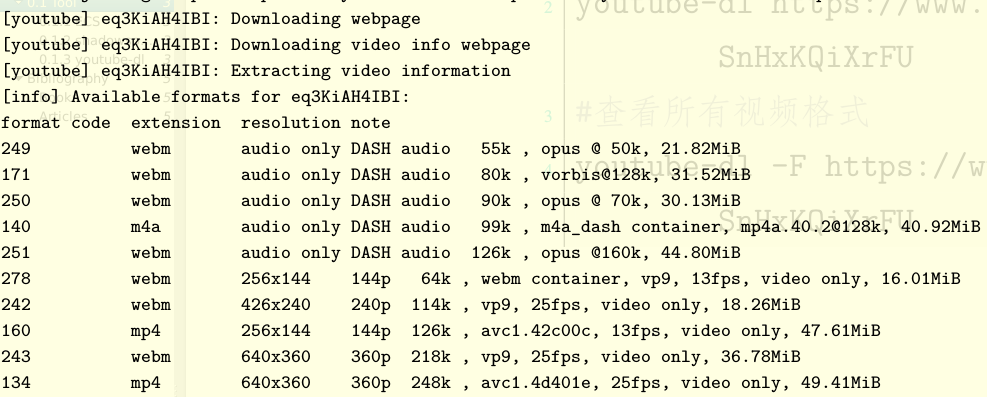
\includegraphics[scale=0.4]{checkyoubevideoformat.png}
	\caption{查看所有格式视频}
	\label{fig:checkyoubevideoformat}
\end{figure}




%----------------------------------------------------------------------------------------
%	CHAPTER 1
%----------------------------------------------------------------------------------------

\chapterimage{chapterhead2.pdf} % Chapter heading image


\subsection{Jenkins}

启动Jenkins提示Job for jenkins.service failed because the control process exited with error code. See "systemctl status jenkins.service" and "journalctl -xe" for details。多半是由于Java未安装或者安装后未指定Java路径。打开文件:

\begin{lstlisting}[language=bash]
#配置文件中指定Java路径
vim /etc/rc.d/init.d/jenkins
#启动Jenkins
service jenkins start
\end{lstlisting}

配置文件中指定Java路径如图所示。

\begin{figure}[htbp]
	\centering
	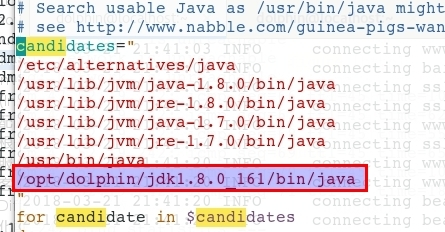
\includegraphics[scale=0.5]{specifyjavapath.jpg}
	\caption{指定Jenkins的Java路径}
	\label{fig:specifyjavapath}
\end{figure}


\subsection{OpenVPN}

OpenVPN从2001年开始开发,使用的是C语言。此处使用的OpenVPN版本是2.4.1。如果使用Mac下的brew工具安装,则OpenVPN目录在:/usr/local/Cellar/openvpn/2.4.1,OpenVPN的配置文件在:/usr/local/etc/openvpn。目前OpenVPN能在Solaris、Linux、OpenBSD、FreeBSD、NetBSD、Mac OS X与Microsoft Windows以及Android和iOS上运行,并包含了许多安全性的功能。此处的服务器使用的是CentOS 7.3,客户端包含Fedora 24、Ubuntu 14.04、Ubuntu 16.04、Window 7、Windows 10。在OpenVPN网络中查看存活的主机:

\begin{lstlisting}[language=bash]
nmap -A -T4 10.0.0.*
\end{lstlisting}

\paragraph{安装(Install)}

安装基础包:

\begin{lstlisting}[language=bash]
sudo yum -y install openssl openssl-devel lzo openvpn easy-rsa --allowerasing
#手动安装
wget -c https://swupdate.openvpn.org/community/releases/openvpn-2.4.1.tar.gz
tar -zxvf openvpn-2.4.1.tar.gz
./configure
make && make install
\end{lstlisting}

LZO 是致力于解压速度的一种数据压缩算法,LZO 是 Lempel-Ziv-Oberhumer 的缩写。这个算法是无损算法,参考实现程序是线程安全的。 实现它的一个自由软件工具是lzop。最初的库是用 ANSI C 编写、并且遵从 GNU通用公共许可证发布的。现在 LZO 有用于 Perl、Python 以及 Java 的各种版本。代码版权的所有者是 Markus F. X. J. Oberhumer。如果没有安装easyrsa工具,使用如下命令安装:

\begin{lstlisting}[language=Bash]
#下载easy-rsa源码
wget -c https://github.com/OpenVPN/easy-rsa/archive/master.zip
#目录/etc/openvpn/easy-rsa/easyrsa3下拷贝默认配置
cp var.example vars
\end{lstlisting}


\paragraph{调整配置}

修改证书生成的配置文件:

\begin{lstlisting}[language=Bash]
set_var EASYRSA_REQ_COUNTRY     "CN"
set_var EASYRSA_REQ_PROVINCE    "Chongqing"
set_var EASYRSA_REQ_CITY        "Chongqing"
set_var EASYRSA_REQ_ORG "Three people"
set_var EASYRSA_REQ_EMAIL       "jiangtingqiang@gmail.com"
set_var EASYRSA_REQ_OU          "My Organizational"

set_var EASYRSA_KEY_SIZE        2048
\end{lstlisting}

\paragraph{生成根证书}

生成OpenVPN的根证书:

\begin{lstlisting}[language=Bash]
#清除之前生成的证书,重新生成;
./easyrsa clean-all
#生成root根证书
#证书路径:/etc/openvpn/easy-rsa/easyrsa3/pki/ca.crt
./easyrsa build-ca
\end{lstlisting}


\paragraph{生成服务器端证书}

生成服务器端证书命令如下:

\begin{lstlisting}[language=Bash]
# 指定服务端证书的文件名为server,可以任意改动
./easyrsa build-server-full server
\end{lstlisting}


\paragraph{生成客户端证书}

生成客户端证书端步骤如下:

\begin{lstlisting}[language=Bash]
./easyrsa build-client-full jiangxiaoqiang
\end{lstlisting}

PKI:Public Key Infrastructure公钥基础设施。生成请求:

\begin{lstlisting}[language=Bash]
./easyrsa gen-req dolphinfedora
\end{lstlisting}

输入PEM验证码。PEM - Privacy Enhanced Mail,打开看文本格式,以"-----BEGIN..."开头, "-----END..."结尾,内容是BASE64编码。
Apache和*NIX服务器偏向于使用这种编码格式.签约:

\begin{lstlisting}[language=Bash]
#切换到服务端生成rsa的目录
#导入req
./easyrsa import-req ~/client/easyrsa/easy-rsa-master/easyrsa3/pki/reqs/dolphinfedora.req dolphinfedora
#用户签约,根据提示输入服务端的ca密码
./easyrsa sign client dolphinfedora
\end{lstlisting}

PKI:Public Key Infrastructure公钥基础设施。输入PEM验证码。PEM - Privacy Enhanced Mail,打开看文本格式,以"-----BEGIN..."开头, "-----END..."结尾,内容是BASE64编码.查看PEM格式证书的信息:openssl x509 -in certificate.pem -text -noout。Apache和*NIX服务器偏向于使用这种编码格式.服务端生成的文件有:

\begin{tabular}{|c|p{5cm}|c|}
	\hline
	\multirow{1}{*}{文件名称}
	& \multicolumn{1}{c|}{说明(Purpose)} 
	& \multicolumn{1}{c|}{位置} \\			
	\cline{1-3}
	ca.crt  & 根证书(Root CA certificate)件 & Server+All Clients	\\
	\hline
	reqs/server.req  & &\\
	\hline
	reqs/dolphin.req  & &\\
	\hline
	private/ca.key & 根证书私钥(Root CA key) & key signing machine only\\
	\hline
	private/server.key && \\
	\hline
	issued/server.crt & 服务器证书Server Certificate & server only\\
	\hline
	issued/dolphin.crt && \\
	\hline
	dh.pem & Diffie Hellman parameters & server only \\
	\hline
\end{tabular}

客户端生成的文件有:

\begin{tabular}{|c|p{8cm}|c|}
	\hline
	\multirow{1}{*}{序号}
	& \multicolumn{1}{c|}{名称}  \\			
	\cline{1-2}
	private/dolphinclient.key  & \\
	\hline
	reqs/sdolphinclient.req & \\
	\hline
\end{tabular}

拷贝出客户端证书文件:

\begin{lstlisting}[language=Bash]
cp easyrsa/easy-rsa-master/easyrsa3/pki/ca.crt ~/dolphinfedora/
cp easyrsa/easy-rsa-master/easyrsa3/pki/issued/dolphinfedora.crt ~/dolphinfedora/
cp ~/client/easyrsa/easy-rsa-master/easyrsa3/pki/private/dolphinfedora.key ~/dolphinfedora/
\end{lstlisting}


启动OpenVPN:

\begin{lstlisting}[language=Bash]
sudo openvpn server.conf
# Mac下启动OpenVPN
sudo /usr/local/Cellar/openvpn/2.4.1/sbin/openvpn /usr/local/etc/openvpn/client.conf
# 需要以后台交互方式启动时
screen sudo openvpn client.conf
\end{lstlisting}

客户端端配置如下:

\begin{lstlisting}[language=Bash]
client         #指定当前VPN是客户端
dev tun        #必须与服务器端的保持一致
proto udp      #必须与服务器端的保持一致
#指定连接的远程服务器的实际IP地址和端口号
remote 192.168.1.106 1194      
#断线自动重新连接
#在网络不稳定的情况下(例如:笔记本电脑无线网络)非常有用
resolv-retry infinite
nobind         #不绑定特定的本地端口号
persist-key
persist-tun
ca ca.crt      #指定CA证书的文件路径
cert client1.crt       #指定当前客户端的证书文件路径
key client1.key    #指定当前客户端的私钥文件路径
ns-cert-type server      #指定采用服务器校验方式
#如果服务器设置了防御DoS等攻击的ta.key
#则必须每个客户端开启;如果未设置,则注释掉这一行;
tls-auth ta.key 1     
comp-lzo              #与服务器保持一致
#指定日志文件的记录详细级别,可选0-9,等级越高日志内容越详细
verb 3                
\end{lstlisting}

配置ns-cert-type(Netscape Cert Type)指定为server主要是防止中间人攻击(Man-in-the-Middle Attack)。在服务端做如下配置:

\begin{lstlisting}[language=Bash]
nsCertType server
\end{lstlisting}

\paragraph{生成Diffle Hellman参数}

生成Diffle Hellman参数命令如下:

\begin{lstlisting}[language=Bash]
./easyrsa gen-dh
\end{lstlisting}

\paragraph{初始化配置文件}

初始化配置文件如下:

\begin{lstlisting}[language=Bash]
#拷贝示例配置到配置目录
cp /usr/share/doc/openvpn-2.4.4/sample/sample-config-files/server.conf /etc/openvpn
\end{lstlisting}

拷贝server.crt/ca.cert等文件到配置目录.


\paragraph{生成ta.key}

使用如下命令生成ta.key:

\begin{lstlisting}[language=Bash]
openvpn --genkey --secret ta.key
\end{lstlisting}

启动服务端:

\begin{lstlisting}[language=Bash]
openvpn --config /etc/openvpn/server.conf
\end{lstlisting}

\subsection{fastDFS}

启动tracker server:

\begin{lstlisting}[language=Bash]
/usr/bin/fdfs_trackerd /etc/fdfs/tracker.conf
\end{lstlisting}

启动storaged server:

\begin{lstlisting}[language=Bash]
/usr/bin/fdfs_storaged /etc/fdfs/storage.conf
\end{lstlisting}




\part{DB}


\chapter{MariaDB}

\section{常用操作}

在CentOS下启动MariaDB:

\begin{lstlisting}[language=Bash]
systemctl start mariadb.service
\end{lstlisting}


\subsection{导入导出}

导出整个库结构和数据:

\begin{lstlisting}[language=Bash]
mysqldump -h localhost -uroot -p123456  database > dump.sql
\end{lstlisting}

启动MariaDB时注意是否带了--skip-networking参数,否则会出现数据库启动了,但是端口没有监听的情况。

\paragraph{允许远程登录}

首先以root用户登陆MariaDB服务器:

\begin{lstlisting}[language=Bash]
--允许用户名为`dolphin`的用户从任意ip以密码为123456访问所有数据库
grant all PRIVILEGES on *.* to dolphin@'%' identified by '123456';
--使其生效
flush privileges;
\end{lstlisting}

\paragraph{修改数据库密码}

修改数据库密码如下:

\begin{lstlisting}[language=Bash]
#登录SQL
mysql -uroot -p
use mysql;  
UPDATE user SET password=password('newpassword') WHERE user='root';  
flush privileges;  
exit;
\end{lstlisting}






\section{常见问题}

\subsection{mariadb 1045 (28000): Access denied for user 'root'@'localhost' (using password: YES)}

在使用命令登录时,出现错误.依次执行如下语句即可:

\begin{lstlisting}[language=Bash]
#停止MariaDB
systemctl stop mariadb.service
#登录
mysqld_safe --user=mysql --skip-grant-tables --skip-networking &
mysql -u root mysql
#设置新密码
UPDATE user SET Password=PASSWORD('123123') where USER='root'; 
FLUSH PRIVILEGES;
quit
#启动MariaDB
systemctl start mariadb.service
\end{lstlisting}

修改后,登录数据库:

\begin{lstlisting}[language=Bash]
mysql -u root -p123123
\end{lstlisting}


\chapter*{Bibliography}
\addcontentsline{toc}{chapter}{\textcolor{ocre}{Bibliography}}
\section*{Books}
\addcontentsline{toc}{section}{Books}
\printbibliography[heading=bibempty,type=book]
\section*{Articles}
\addcontentsline{toc}{section}{Articles}
\printbibliography[heading=bibempty,type=article]

%----------------------------------------------------------------------------------------
%	INDEX
%----------------------------------------------------------------------------------------

\cleardoublepage
\phantomsection
\setlength{\columnsep}{0.75cm}
\addcontentsline{toc}{chapter}{\textcolor{ocre}{Index}}
\printindex

%----------------------------------------------------------------------------------------

\end{document}
